% !TeX root = ../handout.tex

\section{Social Linked Data}

Eine mögliche Implementierung des Data Space Konzepts basiert auf \emph{Social Linked Data} (Solid), welches das Ziel verfolgt, ein Fundament für offene, dezentralisierte Netzwerke für einen souveränen Datenaustausch zu schaffen.
Solid definiert dazu Protokolle für die Verwaltung und den Austausch von Daten in einer dezentralisierten Umgebung, welche auf W3C"=Empfehlungen basiert~\cite{mecklerWebLinkedData2023}.

% Im folgenden Abschnitt wird ein Solid getriebenes Data Space Konzept sowie Solid"=Anwendungen erläutert.
% Darauf aufbauend werden die Konzepte der Identität und Authentifizierung sowie das Datenmanagement und der Datenaustausch in Solid betrachtet.
% Abschließend wird eine Erweiterung von Solid vorgestellt, welche die Ermöglichung von B2B"=Datenwertschöpfungsketten zum Ziel hat.


% \subsection{Solid Data Spaces}

% Solid Data Spaces
Solid Data Spaces verwenden die Web"=Architektur in Kombination mit Solid zur Bildung von Data Spaces.
Dabei werden existierende Web"=Technologien erweitert, um eine Umgebung für sicheres Data Sharing zu erschaffen~\cite{mecklerWebLinkedData2023}.
Dafür werden Anwendungen in drei Teile gegliedert: die (1) Anwendung als solches, (2) Daten und (3) Identität (vgl. \autoref{fig:solid-components}).

% Komponenten
Die Identitätskomponente (3) verifiziert die Identität eines Akteurs zur Authentifizierung zum Datenzugriff.
Die Daten und zugehörigen Zugriffsregeln (2) werden dezentral in einem oder mehreren sog. \emph{Personal Online Data Stores} (Pods) gespeichert.
Eine Anwendung (1) verwendet (3), um den korrekten Pods zu identifizieren und sich für den Datenzugriff zu authentifizieren.
Nach erfolgreicher Authentifizierung, kann eine Anwendung die erforderlichen Daten aus den Pods lesen und schreiben.
Solid definiert dabei den \emph{Access"=Layer}, d.h. die Protokolle zur Verwaltung von Daten und Identitäten sowie die Zugriffskontrolle.
Durch die Trennung, Standardisierung und somit Austauschbarkeit der einzelnen Komponenten ist eine Schritt"=für"=Schritt"=Einführung möglich, wodurch die Einstiegsbarriere gering gehalten und dadurch die Zugänglichkeit erhöht werden kann~\cite{mecklerWebLinkedData2023}.

\begin{figure}[b]
    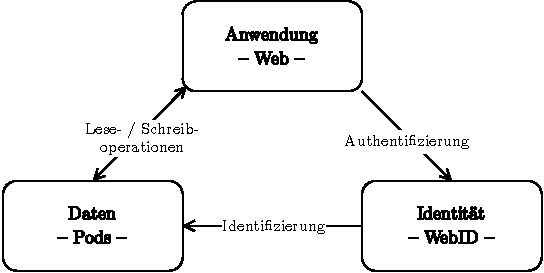
\includegraphics[width=0.7\textwidth]{./assets/solid_triangle.drawio.pdf}
    \caption{Komponenten von Solid}
    \label{fig:solid-components}
\end{figure}


\subsection{Datenmanagement und Datenzugriff}

Daten werden, entsprechend des Data Space Konzepts, dezentral in sog. \emph{Personal Online Data Stores} (Pods) und nicht zentral bei den Anwendungen gespeichert~\cite{mecklerWebLinkedData2023}.
Durch die Verwendung von Standards kann somit eine Interoperabilität auf der Daten"= statt der Anwendungsebene erzeugt werden, wodurch ein einfacher Wechsel von Anwendungen ohne aufwendige Datenmigration möglich ist.

% Datenstruktur
Da Binärdateien schlecht maschinell lesbar und somit schlecht automatisiert verarbeitbar sind, müssen zusätzliche Metadaten gespeichert werden.
Ein lesbares Format für Mensch und Maschine ist jedoch anzustreben, um eine höhere Effizienz durch Automatisierung zu ermöglichen.
Dafür wird das \emph{Resource Description Framework} (RDF) in Kombination mit \emph{Vocabularies} verwendet.
Durch eine Verknüpfung nach dem \emph{Linked Data} Ansatz entstehen strukturierte Daten mit einer automatisierbaren Semantik, welche mit verwandten Ressourcen vernetzt sind~\cite{bizerLinkedDataStory2009,mecklerWebLinkedData2023,sambraSolidPlatformDecentralized2016}.
% TODO: Mesh-Gedanke
Andere Datenstrukturen können mittels Mapping zu RDF oder als Binärdateien mit zusätzlichen Metadaten zur Speicherung der Semantik in Pods integriert werden~\cite{mecklerWebLinkedData2023,sambraSolidPlatformDecentralized2016}.

Die Daten werden in Form von \emph{LDP"=Containern} gespeichert.
Diese sind an sich selbst ein RDF"=Graph, wodurch eine Hierarchie durch Verschachtelung möglich ist (vgl. Verzeichnisstruktur).
Auf jeder Ebene der Hierarchie kann eine Zugriffskontrolle über \emph{Access Control List} (ACL) Ressourcen definiert werden.
Es können unterschiedliche Rechte pro Akteur sowie pro Ressource bzw. Container eingerichtet werden, wodurch feingranularer Datenschutz gewährleistet werden kann~\cite{mecklerWebLinkedData2023,sambraSolidPlatformDecentralized2016}.

% Lesen und Schreiben
Solid"=Anwendungen lesen und schreiben Daten direkt von und in den Pods.
Da Pods interoperabel mit den Anwendungen sein müssen, um eine Austauschbarkeit zu gewährleisten, muss ein wohldefiniertes und möglichst einfach implementierbares Protokoll zum Datenzugriff eingesetzt werden.
Solid verwendet dafür RESTful"=Methoden basierend auf der \emph{Linked Data Platform} (LDP).
Diese definiert bestimmte HTTP"=Operationen auf Web"=Ressourcen, wodurch alle CRUD"=Operationen abgedeckt werden.
Um eine Ressource global eindeutig zu identifizieren, ist jeder Ressource ein \emph{Uniform Resource Identifier} (URI) zugewiesen~\cite{mecklerWebLinkedData2023,sambraSolidPlatformDecentralized2016}.

% SPARQL
Mit den LDP"=Methoden sind jedoch nur einfache Anfragen möglich.
Komplizierte Datenabfragen können optional mittels SPARQL unterstützt werden.
Um den Entwicklungsaufwand zu verringern, werden diese Operationen an den Server delegiert.
Dabei sind \emph{Local Queries}, welche nur innerhalb \emph{eines} Pods operieren, und \emph{Link Following Queries}, welche über mehrere Pods hinweg mittels Verfolgung von Links operieren, möglich.
Die tatsächliche Verteilung muss dabei nicht bekannt sein~\cite{sambraSolidPlatformDecentralized2016}.


\subsection{Identität und Authentifizierung}

Um Vertrauen, Datensouveränität und Datenschutz zu gewährleisten ist eine Authentifizierung von Akteuren notwendig.
Zum Erreichen einer Dezentralisierung ist ein globaler \emph{Identity Space} notwendig, welcher zur RDF"=basierten Daten in den Pods sowie der gewünschten Erweiterbarkeit passt und relevante Links zu den Datenspeichern liefert.
\emph{WebID} erfüllt die genannten Kriterien und wird daher in Solid verwendet~\cite{sambraSolidPlatformDecentralized2016}.

Akteure besitzen eine WebID"=URI, welche ein \emph{WebID Profile Document} referenziert.
Dieses enthält wiederum Referenzen auf den Pod und die Anwendungsdaten sowie weitere Dokumente, um das Profil zu beschreiben~\cite{solidcommunitygroupSolidWebIDProfile2024}.
Das Profile Document wird bei einem \emph{Identity Provider} (meist Pod Provider) gespeichert, wodurch die Akteure die Kontrolle über die eigene Identität behalten~\cite{sambraSolidPlatformDecentralized2016}.

Eine Besonderheit bei Solid ist, dass sich Akteure gegenüber Anwendungen nicht authentifizieren müssen.
Eine Authentifizierung wird ggf. nur durchgeführt, um die WebID des Akteurs zu erlangen.
Anschließend wird eine Authentifizierung nur zwischen dem Browser und den relevanten Pods durchgeführt~\cite{sambraSolidPlatformDecentralized2016}.

Durch die Möglichkeit, Identitäten über mehrere Seiten hinweg zu verknüpfen, entsteht ein \emph{Web of Trust}.
Dies ermöglicht es, Authentifizierungsentscheidungen ad-hoc basierend auf den Eigenschaften der Akteure, wie bspw. den Beziehungen zu anderen Akteuren, zu treffen~\cite{sambraSolidPlatformDecentralized2016}.
Auf dieser Basis kann entschieden werden, wem vertraut werden kann, mit wem ein vertrauenswürdiger Datenaustausch möglich ist und ob den geteilten Daten vertraut werden kann.
Somit wird ein großes Hindernis des Data Sharings direkt adressiert.


\subsection{Erweiterung: B2B-Wertschöpfungsketten}

Eine automatisierte Datenübertragung ist essenziell für Partner in einer Wertschöpfungskette, ist jedoch an weitere Anforderungen geknüpft.
So müssen bspw. rechtliche Rahmenbedingungen garantiert und nachvollziehbar eingehalten werden.
Solid bietet dafür bereits eine Grundlage, ist aber noch nicht ausreichend.
Weitere Metadaten sind notwendig, um \emph{Constraints} für das Data Sharing zu etablieren~\cite{bothSolidBasedB2BData2025}.

Zum einen kann über Metadaten ein \emph{Data Processing Purpose} angegeben werden, welche die minimal möglichen und notwendigen Rechte beschreibt.
Die Weitergabe von Daten soll nur unter mindestens genauso starken Restriktionen erlaubt sein.
Dafür führt \cite{bothSolidBasedB2BData2025} eine Purpose"=Klassen ein, welche weitergegeben werden muss~\cite{bothSolidBasedB2BData2025}.

Andererseits soll die ursprüngliche Quelle bei der Weitergabe von Daten versteckt werden.
Um eine spätere Nachvollziehbarkeit zu garantieren, soll jedoch angegeben werden, dass die Zugriffsrechte und weitergegebenen Daten auf einer Freigabe durch eine Drittpartei basiert.
Dies wird durch eine \emph{Facade}"=Klasse umgesetzt, welche den ursprünglichen Data Provider versteckt~\cite{bothSolidBasedB2BData2025}.

Diese Erweiterung zeigt die Möglichkeiten und Notwendigkeiten der Erweiterbarkeit von Solid.
Sie dient als weiterer Schritt in Richtung E2E"=B2B"=Wertschöpfungsketten unter der Berücksichtigung des Schutzes von Daten und Geschäftsgeheimnissen.
Allerdings ist weitere Forschung notwendig, um die verwendete Purpose"=Ontologie zu validieren, um vollständig automatisierbare Prozesse zu etablieren~\cite{bothSolidBasedB2BData2025}.
